\documentclass[../main.tex]{subfiles}
\begin{document}
\subsection{Условие применимости метода линеаризации в задаче локального синтеза} 
We consider the problem of a feedback control design for a nonlinear control-affine system. The aim of the control is to bring  trajectories of the closed system to the origin of coordinates in a given time, providing the minimal value of an integral functional. The object under study is the nonlinear system, closed by a linear feedback controller. The controller is  obtained as a solution of the LQR problem for the linearized system. We indicate sufficient conditions  for this linear feedback to give a local solution to the control synthesis problem under consideration.  In addition, we give some  error estimates for the values of the functional. 

\subsubsection{Introduction}

We propose here a method for solving the problem of a local control synthesis  for a control-affine system on a small time interval. This method is based  on the linearization of the original nonlinear system in the vicinity  of the equilibrium position.  Linearization is often used in solving various control problems, such as stabilization problems\cite{Kras_add,Khalil}, stochastic and numerical control\cite{Roxin,EKF,denBerg,Pang}, MPC control\cite{Murillo,LTV_MPC}, etc.

In this article, we study the problem of control synthesis with an integral quadratic cost. Note that the task is considered on a finite, and, moreover, small, time interval. The goal of the control is to transfer the system to the origin in a given time ensuring the minimum value of the cost. The linear feedback control found for the linearized system is used as  the input of the original non-linear system. For a linear control system the optimal feedback is linear in state, with gains increasing indefinitely when approaching the terminal time. The latter  makes it difficult to justify the applicability of the linearization method. The restrictions on  asymptotics  of the controllability Gramian of the linearized system are needed in this case. Unlike, for example, the stabilization problem for which controllability (stabilizability) of the linearized system implies stabilizability of the nonlinear system. These restrictions coincide with the  asymptotic equivalence conditions for reachable  (null-controllable) sets of nonlinear and linearized systems. In \cite{GusevOsipov} it was shown that, under these conditions the control in the form of a linear state feedback takes all trajectories starting from some neighborhood of zero to zero, if the control time interval is sufficiently small. 

In this article, we generalize the main result of \cite{GusevOsipov}. The proposed sufficient conditions have the form of an inequality for some improper integral. They depend on the smallest and the largest eigenvalues of the controllability Gramian of the linearized system and contain a scalar parameter. The choice of this parameter makes it possible to cover a wider class of control systems, the conditions from \cite{GusevOsipov} are obtained here as a special case for a certain value of the parameter.

For a linearized system, the considered linear controller delivers the minimum value to the integral functional for any initial state. For a nonlinear system, this is not the case, so it is important to obtain an estimate of the resulting error. This was done in the second part of the article, where  the relation between the values of the integral cost for the trajectories of the nonlinear and linearized systems was studied and  the estimate for the relative error was given. 

The article is structured as follows. The problem statement and some preliminary results are given in the second section. The third section contains the formulation and proof of the main results. Finally, we provide two illustrative examples in the fourth section.

\subsubsection{Постановка задачи}

Рассмотрим нелинейную систему, аффинную по управлению
\begin{gather}\label{sec22:nonlinear}
	\dot{z}(t)=f(z(t))+B u(t),\qquad 0 \leqslant t \leqslant T, \qquad z(0) = z_0.
\end{gather}
 где $ x \in \mathbb{R}^n $ --- вектор состояния, $ u \in \mathbb{R}^r $ --- вектор управления, а $ 
T$ --- некоторое положительное число. 
Будем считать, что функция $f$ обладает следующим свойством.
\begin{property}\label{prop:Residial_term_bounds}
	 Найдутся такие  $r>0$, $k>0$  что при всех $ z \in B(0,r) $, функция  $f(z)$ может быть представлена в форме  $ f(z) = Az + R(z) $, причем  $ \|R(z) \| \leqslant k \| z\|^2  $. 
\end{property}
Здесь $ B(0,r) $ --- это шар радиуса $r$  с центром в точке $0 \in \mathbb{R}^n$. 
Это свойство выполняется, если if $f(0) = 0 $, $\frac{\partial f}{\partial x}(0) 
= A $ и $f(z)$ дважды дифференцируема. 

Напомним, что пространство скалярных или векторных функций интегрируемых с квадратом  на $ [0,T] $ обозначаются через $ \mathbb{L}_2 = \mathbb{L}_2[0,T] $. Шар в пространстве $\mathbb{L}_2$ обозначим через $B_{\mathbb{L}_2}(0,r)$. В качестве функционала мы рассматриваем 
\begin{gather}\label{cost}
		I(T,u):=\int_0^Tu^\top (t)u(t)dt= 	\lVert u(\cdot)\rVert^2_{\mathbb{L}_2.} 
\end{gather}
Задача состоит в синтезе закона управления $u(t)=u(t,z(t))$ который бы приводил траектории замкнутой системы  
\begin{gather*}
	\dot{z}(t)=f(z(t))+B u(t,z(t)),\qquad 0 \leqslant t \leqslant T, \qquad z(0) = z_0.
\end{gather*}
в начало координат за время $T$ и обеспечивал при этом минимальное значение $I(T,u)$. 

Рассмотрим линейный случай ($R(z)=0$)
\begin{gather}\label{sec22:linear}
	\dot{z} =  A  z + B u, \qquad 0 \leqslant t \leqslant T.
\end{gather}
Если система \eqref{sec22:linear} управляема, то решение описанной выше задачи --- это линейный по состоянию закон управления 
\begin{gather}\label{linear_feedback}
	u(t,z) = -B^{\top} Q_T(t) z
\end{gather}
(см, например, \cite{Abgar,Kur1,GusevOsipov}).
Здесь $Q_T(t)=W^{-1}(T-t)$, а $W(t)$ --- грамиан управляемости системы $\dot{x} = -A x - B u$:
\begin{gather*}
    W(t) = \int_0^t e^{-A\tau}BB^\top e^{-A^{\top}\tau}d\tau. 
\end{gather*}
Грамиан $W(t)$ положительно определен при $t>0$ тогда и только того, когда   
система \eqref{sec22:linear} управляема. Можно показать, что $Q_T(t)$ --- решение дифференциального уравнения 
\begin{gather}\label{eqQ}
	\dot{Q_T}  = Q_T B B^{\top} Q_T - A^{\top}Q_T - Q_T A, \quad Q_T(0)=W^{-1}(T).
\end{gather}
Таким образом, чтобы найти $Q_T(t)$ на $(0,T]$, нужно сначала вычислить $W(T)$, а затем проинтегрировать систему \eqref{eqQ}.
Поскольку $W(0)=0$, $Q_T(t)$ определена для $t<T$ и $\|Q_T(t)\| \to \infty$ при $t\to T$. 

Верно следующее утверждение \cite{Abgar,Kur1,GusevOsipov}.
\begin{utv}
Любая траектория $z(t)$ системы \eqref{sec22:linear} с управлением  \eqref{linear_feedback} выходящая из точки  $ z_0 $ достигает начала координат за время $T$. При этом интегральный функционал $I(T,u)$ принимает минимальное значение $z^{\top}_0 Q_T(0) z_0 $ при каждом $z_0$.
\end{utv}
Далее мы будем исследовать поведение траекторий системы \eqref{sec22:nonlinear} замкнутой линейной обратной связью $ u(t,z) = -B^{\top} Q_T(t) z$ при условии, что  $T$ достаточно мало. 
Верно ли, что все траектории, начинающиеся в некоторой окрестности начала координат, достигают его?  
Можно ли что-то сказать о значении интегрального функционала? 

\subsubsection{Асимптотическая эквивалентность множеств достижимости}

Далее, мы будем использовать понятие асимптотической эквивалентности множеств, введенное в разделе \ref{sec21:AsymptoticEquality}. 
Рассмотрим систему, уравнения которой получаются из \eqref{sec22:nonlinear} обращением времени. Положив $\tau=T-t$ мы имеем
\begin{gather}\label{nonlinear_}
			\dot{x}(\tau)=-f(x(\tau))-B v(\tau),\qquad 0 \leqslant \tau \leqslant T; 
\end{gather}
здесь $x(\tau)=z(T-\tau)$, $v(\tau)=u(T-\tau)$.
При заданном $\mu>0$ обозначим через $ G_{-} (T,\mu)$ множество достижимости системы \eqref{nonlinear_} с интегральными квадратичными ограничениями на управление, $G_{-}(T,\mu)=\{x\in \mathbb{R}^n:\exists v(\cdot)\in B_{\mathbb{L}_2}(0,\mu),\; x=x( T,v(\cdot)))\}$.
		 
Здесь $x( \tau,v(\cdot)))$ обозначает решение системы  \eqref{nonlinear_} с нулевыми начальными условиями. 
Свойства множеств достижимости нелинейных систем с интегральными ограничениями на управление изучались во многих работах (см., например, \cite{Guseinov,Rousse,GusZykIFAC}).
Рассмотрим также линейную систему 
\begin{gather}\label{linear_}
			\dot{x}(\tau)=-Ax(\tau)-B v(\tau),\qquad 0 \leqslant \tau \leqslant T; 
\end{gather}
эта система является линеаризацией системы  \eqref{nonlinear_} в начале координат. 
Множество достижимости этой системы обозначим через $G_{-}^0(T,\mu)$. 
Это множество --- эллипсоид в $\mathbb{R}^n$, описываемый неравенством $G_{-}^0(T,\mu)=\{x \in \mathbb{R}^n: x^\top W^{-1}(T)x\leqslant \mu^2\}$.			

%Let $X,Y \subset \mathbb R^n $ be convex compact sets such that the origin is an interior point of both the sets.
%\begin{definition}[see, for example, \cite{Lassak,Ovs}]
%The Banach-Mazur distance between $X$ and $Y$  is defined as
%$\rho(X,Y):=\log\big(r(X,Y)\cdot r(Y,X)\big)$, where \\ $r(X,Y)=\inf \{t\geqslant1:tX \supset Y\}$. 
%\end{definition} 
%From the definition it follows that for any $c>0$, $\rho(cX,cY)=\rho(X,Y)$ and two inclusions are valid: $X\subset \exp(\rho(X,Y))Y$ and $Y\subset \exp(\rho(X,Y))X$.

%Assume that  $X,Y$ depend on a small positive parameter $\tau$,  $0<\tau\leqslant\tau_0$  and set-valued mappings  $X(\tau), Y(\tau)$ are bounded. 
%\begin{definition}[\cite{Ovs}]	
% The sets $ X (\tau), Y (\tau) $ are called asymptotically equal under $\tau \to 0$ if $ \rho (X (\tau), Y (\tau)) \to 0,\;\; \tau \to 0$.
%\end{definition}
Через$\nu(\tau), \eta(\tau)$ обозначим наименьшее и наибольшее собственное число $W(\tau)$ соответственно. Из результатов  \cite{Polyak2001,GusOsSteklov,Osipov,GusevMotor} следует, что множества достижимости  
$G_{-}(\tau,\mu)$ and $G_{-}^0(\tau,\mu)$ асимптотически эквивалентны при $\tau \to 0$ если пара  $(A,B)$ --- управляема 
и существуют такие $ l > 0$, $\tau_0 > 0$ и $\alpha > 0$ что для всех $0 < \tau \leqslant \tau_0 $
		\begin{gather}\label{gramas}
			\nu(\tau)\geqslant l\tau^{4-\alpha}.
		\end{gather}

\begin{zam}
    Множество достижимости $G_{-}(T,\mu)$ системы \eqref{nonlinear_} совпадает с множество нуль-управляемости системы \eqref{sec22:nonlinear}, т.е. множетсва таких начальных условий, из которых система может быть переведена в начало координат управлениями из $B_{\mathbb{L}_2}(0,\mu) $ за время $T$. 
    То же самое справедливо для систем \eqref{linear_} и \eqref{linear_} и соответствующих им множеств $G_{-}^0(T,\mu)$.
\end{zam}

\subsubsection{Задача синтеза управления. Асимптотика траекторий}

Везде ниже мы предполагаем, что пара $A,B$ является управляемой, не уточняя это отдельно.

В этом разделе мы исследуем асимптотическое поведение траекторий системы \eqref{sec22:nonlinear}, замкнутой линейной обратной связью $ u(t,z) = -B^{\top} Q_T(t) z$:
\begin{equation}\label{nonlinear_closed}
	\dot{z} = f(z) - B B^{\top} Q_T(t) z, \qquad 0 \leqslant t \leqslant T, \qquad z(0) = z_0.
\end{equation}
Напомним, что это управление приводит траектории линейной системы $\dot{z} = A z + B z$ к началу координат в момент времени $T$ и обеспечивает минимальное значение функционала. 
Это значение равно $J_0(T,z_0) =z_0^{\top}Q_T(0)z_0$.

Для анализа траекторий системы \eqref{nonlinear_closed} используем следующую лемму
\begin{lemma}\label{lem:zqz} 
    Пусть $C\in \mathbb{R}^{ n \times n}$ и $D\in \mathbb{R}^{n \times n}$ --- симметричные положительно-определенные матрицы, $C=D^{-1}$. Тогда, для любого $\forall z \in \mathbb{R}^{n}$   
    \begin{gather} \label{eig}
        \frac{1}{\lambda_{max}(D)} \|z\|^2 \leqslant z^T C z \leqslant \frac{1}{\lambda_{min}(D)} \|z\|^2,
    \end{gather}
    где $\lambda_{max}(D)$ и $\lambda_{min}(D)$ --- наибольшее и наименьшее собственное число матрицы $D$.
\end{lemma}
\doc. 
  Следует из факта, что наибольшее и наименьшее собственное число матрицы $C$ равны $1/{\lambda_{min}(D)}$ и $1/{\lambda_{max}(D)}$, соответственно. \hfill $ \square $

Если $C=Q_T(t)=W^{-1}(T-t)$, то $D=W(T-t)$ и неравенство \eqref{eig} принимает вид
\begin{gather*} %\label{eig1}
        \frac{1}{\eta(T-t)} \|z\|^2 \leqslant z^T Q_T(t) z \leqslant \frac{1}{\nu(T-t)} \|z\|^2, \quad 0\leqslant t < T.
    \end{gather*}
\begin{assumption} \label{asm1}   
   Пусть существует $\overline{T}>0$ и непрерывная положительная функция $\varphi(\tau): (0, \overline{T}] \to \mathbb{R}$ такие, что
\begin{equation*}
    0 < \frac{\eta(\tau)}{\sqrt{\nu(\tau)}} \leqslant \varphi(\tau), \qquad 0 < \tau \leqslant \overline{T},\quad \int\limits_0^ {\overline{T}}\varphi(\tau) d\tau<\infty.
\end{equation*} 
\end{assumption}
Введем функцию $\Phi(T): [0, \overline{T}] \to \mathbb{R}$
\begin{equation*}
    \Phi(T)= \int\limits_0^ {T}\varphi(\tau) d\tau,\quad 0 <  T \leqslant \overline{T},\quad  \Phi(0)=0.
\end{equation*} 

Напомним, что $\eta(\tau)$ and $\nu(\tau)$ --- это наименьшее и наибольшее собственные числа $W(\tau)$. 
Далее будем считать систему \eqref{linear_} полностью управляемой, поэтому $\eta(\tau) \geqslant \nu(\tau) \geqslant 0$ при $\tau \geq 0$.
 
Поскольку $\varphi(\tau)$ не обязательно ограничено в нуле, $\Phi(T)$ может принимать значения, равные $+\infty$.
\begin{lemma}%\label{lem:Phi}
Верны следующие свойства $\Phi(T)$:
\begin{enumerate}
 \item Если $\Phi(T) < \infty $ хотя бы для одного $T$, то $\Phi(T) < \infty $ для всех $T \in (0, \overline{T}]$.
\item Если $\Phi(T) < \infty $, то $\Phi(T)$ непрерывная и возрастающая функция на $ [0,\overline{T}]$.
 \end{enumerate}
\end{lemma}
\doc. Следует из свойств несобственных интегралов. \hfill $ \square $
\begin{assumption}\label{asm2}
Существует такое $ 0 < \beta \leqslant 1$ что $\frac{\sqrt{\eta(T)}}{\Phi^\beta(T)} \to 0$ при $T \to 0$.
\end{assumption}
Если $\Phi(T)$ конечна, то существует не более одного корня уравнения $\Phi(T)=1$ на $(0,\overline{T}]$, обозначим этот корень через $T^*$.   
Если $\Phi(T)<1$ при $T\in (0,\overline{T}]$ положим $T^*=\overline{T}$. 
Очевидно, что для всех  $ 0 < \beta \leqslant 1$,   $\Phi^\beta(T)\geqslant \Phi(T)$ если $T \leqslant T^*$.

При фиксированном $T\in (0, \overline{T}]$ рассмотрим квадратичную форму $V_T(t,z)=z^{\top}Q_T(t)z$.  
\begin{lemma}\label{lem:vest}
 Пусть выполнено \ref{asm1}. Если $T\leqslant T^*$ и $z(t)$ --- такая траектория системы \eqref{nonlinear_closed} что  $z(t)  \in B(0,r)$ при $0<t \leqslant T$ и $V_T(0,z(0))\leqslant 1/(4k^2\Phi^{2\beta}(T))$ для некоторого $0<\beta \leqslant 1$. 
 Тогда 
 \begin{gather*}
    V_T(t,z(t)) \leqslant \frac{1}{k^2\Phi^{2\beta}(T)}, \qquad 0 \leqslant t \leqslant T. 
 \end{gather*}
\end{lemma}
\doc. 
Продифференцировав $V_T$ вдоль траекториии $z(t)$ системы \eqref{sec22:nonlinear}  на интервале $[0, T]$, мы получим
\begin{gather*}
    \frac{d}{dt}V_T(t,z) = \frac{d}{dt}z^{\top}Q_Tz = \dot{z}^{\top} Q_T z + z^{\top} \dot{Q_T} z + z^{\top} Q_T \dot{z} = \\
    =\left(z^{\top} A^{\top} + R^{\top}(z)- z^{\top} Q_T B B^{\top}\right) Q_T z + \\ +
		z^{\top} Q_T \left(A +R(z) - B B^{\top} Q_T\right)z + z^{\top} \left(Q B B^{\top} Q_T - A^{\top}Q - Q_T A \right) z = \\
    = R^{\top}(z)Q_T z + z^{\top} Q_T R(z) - z^{\top} (Q_T B B^{\top} Q_T) z = \\
    = 2 \left( R(z), Q_Tz \right) - z^{\top} Q_T B B^{\top} Q_T z 
\end{gather*}
Хотя здесь $z$ и $Q_T$ зависят от $t$, для краткости мы опускаем явную зависимость в обозначениях.  
Из $z^{\top} Q_T B B^{\top} Q_T z\geqslant 0$, следует, что
\begin{gather}\label{dvt_first}
    \frac{d}{dt}V_T(t,z) \leqslant 2 \left( R(z), Q_T z\right)=2(R(z),z)_{Q_T} \leqslant 2 \| R(z) \|_{Q_T} \| z \|_{Q_T}.
\end{gather}
Здесь использованы обозначения $(x,y)_{Q_T}=x^\top Q_Ty$ и  $\| x \|_{Q_T} =\sqrt{(x,x)_{Q_T}}$ для $x,y\in \mathbb R^n$. 
Так как $z = z(t) \in B(0,r)$ то, учитывая, что $\|R(z)\| \leqslant k\|z\|^2$  и применяя Лемму \ref{lem:zqz}, получаем 
\begin{equation}\label{rqr_est}
     \| R(z) \|_{Q_T} \leqslant \frac{1}{\sqrt{\nu(T - t)}} \|R(z)\| \leqslant \frac{k}{\sqrt{\nu(T - t)}}\|z\|^2 \leqslant k \frac{\eta(T-t)}{\sqrt{\nu(T-t)}}V_T.
\end{equation}
Напомним, что  $ Q_T^{-1}(t) = W(T-t) $.
Подставляя полученную выше оценку в \eqref{dvt_first} приходим к
\begin{equation}\label{dvt}
    \frac{d}{dt}V_T \leqslant 2 k \frac{\eta(T-t)}{\sqrt{\nu(T-t)}}V_T^{\frc{3}{2}} \leqslant 2k \varphi(T-t) V_T^{\frc{3}{2}}
\end{equation}
Давайте введем систему
\begin{equation}\label{comparison_system}
    \dot{\psi} = 2k \varphi(T-t) \psi,
\end{equation}
которую мы будем использовать как систему сравнения для \eqref{dvt}. 
Проинтегрировав эту систему, мы имеем
\begin{gather*}
    d\psi^{-\frc{1}{2}} = -k \varphi(T-t) dt, \quad
    \psi^{-\frc{1}{2}}(t) = -k \int\limits_0^t \varphi(T-\zeta) d\zeta + C,
\end{gather*}
где
\begin{gather*}
    0 < \int\limits_0^t \varphi(T-\zeta) d\zeta \leqslant \int\limits_0^T \varphi(T-\zeta) d\zeta = 
    \int\limits_0^T \varphi(\tau) d\tau = \Phi(T) 
\end{gather*}
Выберем $C = 2k (\Phi(T))^{\beta}$ then $\psi^{-\frc{1}{2}} \geqslant 2k (\Phi(T))^{\beta} - k \Phi(T) = k (2\Phi^\beta - \Phi)\geqslant k\Phi^\beta $.
%% \\ \frac{2\Phi^\beta - \Phi}{\Phi} = 2 - \Phi^{1 - \beta} \to 2, \mbox{  while } \Phi \to 0   
Тогда $\psi(t) \leqslant \big(k^2\Phi^{2\beta}(T)\big)^{-1}$ для всех $ 0 \leqslant t \leqslant T^* $ и $\psi(0) = \big(4k^2\Phi^{2\beta}(T)\big)^{-1} $.
Таким образом, $V_T(0,z(0))\leqslant \psi(0)$ и теорема сравнения \cite{walter}, примененная к \eqref{dvt}, \eqref{comparison_system}, означает, что выполняется неравенство $V_T(t,z(t))\leqslant \psi(t)$. 
Это завершает доказательство.
	\hfill $ \square $

\begin{theorem}\label{th:tends_to_zero}
    Пусть выполнены предположения \ref{asm1}, \ref{asm2}. Тогда существует такое $ T_1 \leqslant T^*$ что для всех $ T \leqslant T_1$, найдется такой $ r_1(T)$ что траектории системы \eqref{nonlinear_closed} выходящие из $z(0) = z_0 \in B(0,r_1(T))$ стремятся к $0$ при $t \to T$.
\end{theorem}

\doc. 
Поскольку $\frac{\sqrt{\eta(T)}}{\Phi^\beta(T)} $ стремится к $0$ если $T$ стремится к $0$, то найдется такой $ T_1 \leqslant T^*$, что выполняется следующее неравенство
$ \sqrt{\eta(T)}/(k\Phi^\beta(T))  \leqslant r/{2}, \; \forall T \in [0;T_1]$.

Определим $r_1(T)$ равенством
\begin{gather}\label{r1}
    r_1(T) = \min \left\{ \frac{r}{4}, \frac{\sqrt{\nu(T)}}{2k\Phi^\beta(T)} \right\}.
\end{gather}


Здесь нам нужно доказать, что вся траектория $z(t)$ лежит в сфере $B(0,r)$, чтобы использовать оценку \eqref{z_est} из предыдущего раздела. 
Из \eqref{r1} немедленно следует, что  $r_1(T) < r$.  Отсюда и из условий теоремы и  следует, что $z_0 \in B(0,r_1(T)) \subset B(0,r) $. 
Более того, непрерывность траектории  $z(t)$ означает, что условие $z(t) \in B(0,r) $ выполняется и для близких к нулю значений  $t$.  

Обозначим $t^* = \sup \left\{ t: z(t) \in B\left(0,0.5r\right)\right\} $.
Предположим, что $t^* < T$, это означает, что  $z(t) \notin B(0,0.5r)$, при $t > t^*$. Тогда, мы можем выбрать такое положительное  $ \varepsilon$, что включение $z(t) \in B(0,r)$ будет выполняться для всех $0 \leqslant t \leqslant t^* + \varepsilon$. 

Из условия \eqref{r1} следует, что для $0 \leqslant t \leqslant t^* + \varepsilon$ будет выполняться следующее условие
\begin{gather*}
    V_T(0,z_0) \leqslant \frac{1}{\nu(T)} \|z_0\|^2 \leqslant \frac{1}{\nu(T)} r_1^2 \leqslant \frac{1}{4k^2\Phi^{2\beta}(T)}.
\end{gather*}
Из Леммы \ref{lem:vest} вытекает, что  
$V_T(t, z(t))  \leqslant \psi(t) $ и
\begin{gather}\label{z_est}
    \|z(t)\|^2 \leqslant \eta(T-t) V_T(t,z(t)) \leqslant \eta(T-t) \psi(t) \leqslant  \frac{\eta(T)}{k^2\Phi^{2\beta}(T)},
\end{gather}
поэтому, $\|z(t)\| \leqslant \frac{\sqrt{\eta(T)}}{k\Phi^\beta(T)} \leqslant r/2$  для всех $0\leqslant t \leqslant t^*+\varepsilon$,
что противоречит определению $t^*$.  
А значит, включение $z(t) \in B(0,r) $  и неравенство  $V_T(t,z(t)\leqslant \psi(t)$ справедливы для всех $t \in [0; T]$.
        
Наконец, $ \|z(t)\|^2 \leqslant \eta(T-t)\psi(t) \leqslant \eta(T-t)\big(k^2\Phi^{2\beta}(T)\big)^{-1} $, 
где $\eta(T-t) \to 0$ при $t \to T$, а это означает, что $\|z(t)\|$ тоже стремится к нулю.
	\hfill $ \square $
\begin{corollary}%\label{cor:1}
Пусть существуют такие $ l > 0$, $\tau_0 > 0$ и $\alpha > 0$ что для всех $0 < \tau \leqslant \tau_0 $ выполняется
		\begin{gather}\label{asymp}
			\nu(\tau)\geqslant l\tau^{4-\alpha}.
		\end{gather}
 Тогда справедливы Предположения \ref{asm1} и \ref{asm2} и, следовательно, утверждение Теоремы \ref{th:tends_to_zero} является верным.
\end{corollary}
\doc. 
Положим $\overline{T}=\tau_0$. 
Существует такое $m>0$, что $\eta(\tau)\leqslant m \tau$,  для $0 < \tau \leqslant\overline{T}$ (см,например, \cite{GusevOsipov}). 
Следоватльно, имеем $
\eta(\tau)/\sqrt{\nu(\tau)} \leqslant  
	 ml^{-1/2}\tau^{-1+\alpha/2},$
и можем взять  $\varphi(\tau):=  
	 ml^{-1/2}\tau^{-1+\alpha/2}$. 
В этом случае 
$\Phi(T)=2mT^{\alpha/2}/(l^{-1/2}\alpha)$, и Предположение \ref{asm1}, очевидно, выполняется. 
Поскольку 
$\sqrt{\eta(T)}/\Phi^\beta(T) \leqslant c_0T^{(1-\alpha\beta)/2},$
где $c_0$ --- константа, то для выполнения Предполжения  \ref{asm2} достаточно взять $\beta < 1/\alpha$.
	\hfill $ \square $
Заметим, что неравенство \eqref{asymp} совпадает с условием, из которого следует Теорема 1 из \cite{GusevOsipov}.

\subsubsection{Error estimates for the value of cost functional}

In this part  of the paper, we will focus on the value of integral functional \eqref{cost}, when applying linear feedback \eqref{linear_feedback} to a non-linear system \eqref{sec22:nonlinear}. Recall that in the linear case of system \eqref{sec22:linear}, this functional takes the minimum value on the control \eqref{linear_feedback}. We previously denote it by $J_0(T,z_0)$. The designation $J(T,z_0)$ we use for the value of the functional on the trajectory  of system \eqref{nonlinear_closed}.
 In order to obtain an  expression for $J(T,z_0)$ we need to integrate \eqref{dvt_first} from $0$ to $t$:
\begin{gather}\label{J}
	z^{\top}(t) Q_T(t)z(t) = z_0^{\top} Q_T(0)z_0 - \int_{0}^{t} u^{\top}(\xi)  u(\xi) \, d\xi + 2\int_{0}^{t}  R^{\top}(z(\xi))Q(\xi) z(\xi) d\xi,
\end{gather}
    where $ u(\xi) = -B^{\top} Q_T(\xi) z(\xi)$ is a control at time $\xi$. In the linear case, $R(z) \equiv 0$ and $z^{\top}(t) Q_T(t)z(t) \to 0 $ as $t \to T$ so
\begin{gather*}
    J_0(T,z_0) = z_0^{\top} Q_T(0)z_0 = \int_{0}^{t} u^{\top}(\xi)  u(\xi) \, d\xi.
\end{gather*}
Further, we are going to investigate the behaviour of the quadratic form $z^{\top}(t) Q_T(t)z(t) $ and the residual term in \eqref{J}, which we denote by
\begin{gather*}
			\gamma (t,z_0) = 
		 2\int_{0}^{t}  R^{\top}(z(\xi,z_0))Q(\xi) z(\xi,z_0) d\xi.
\end{gather*}

\begin{theorem}\label{th:functional_error_estimate}
  Let Assumption \ref{asm1} be fulfilled. Let $x(t)$ be a trajectory of system \eqref{nonlinear_closed}  such that $x(t)\in B(0,r)$, $0\leqslant t  \leqslant \tilde{T} \leqslant \overline{T} $ and $V_{\tilde{T}}(t,x(t))\to 0$ as $t\to \tilde{T}$. Then there exists $T_2 \leqslant \tilde{T}$ such that for all $0 < T < T_2 $ the following estimate holds
   \begin{gather} \label{est}
	 \left| \frac{	J(T) - J_0(T)}{J_0(T)}\right| \leqslant 16k\Phi({T})J^{1/2}_0(T).
    \end{gather}
    Here $J(T)=J(T,x(\tilde{T}-T))$, $J_0(T)=J_0(T,x(\tilde{T}-T))$ are the values of functional $I(T,u(\cdot))$ on the trajectories of nonlinear and linearized systems accordingly.
\end{theorem}
\doc
Let $T\leqslant \tilde{T}$. Denote by $z(t)$ the trajectory  of system \eqref{nonlinear_closed} with initial state $z(0)=x(\tilde{T}-T)$ on the interval $[0,T)$. Then we have 
\begin{gather*}
Q_T(t)=W^{-1}(T-t)=W^{-1}(\tilde{T}-(\tilde{T}-T+t))=Q_{\tilde{T}}(\tilde{T}-T+t) = Q(\tau), \\ V_T(t,z(t))=z^\top(t)Q_T(t)z(t)=V_{\tilde{T}}(\tau,x(\tau)),
\end{gather*}
where $\tau=\tilde{T}-T+t$. $V_T(0,z(0))=V_{\tilde{T}}(\tilde{T}-T, x(\tilde{T}-T))$, $V_{\tilde{T}}(t,x(t))\to 0$ as $t\to \tilde{T}$. Since  $V_{\tilde{T}}(t,x(t))\to 0$,  $t\to \tilde{T}$ we have that $V_T(0,z(0))=J_0(T)$  tends to zero as $T\to 0$.
Clearly,  $V_T(t,z(t))=z^\top(t)Q_T(t)z(t)=V_{\tilde{T}}(\tau,x(\tau))$ tends to zero as $t\to T$.
Using this, let us rewrite \eqref{J} 
\begin{gather}\label{J1}
	 \int_{0}^{T} u^{\top}(\xi)  u(\xi) \, d\xi - z_0^{\top} Q_T(0)z_0= 2\int_{0}^{T}  R^{\top}(z(\xi))Q(\xi) z(\xi) d\xi=\gamma(T,z(0)),
\end{gather}
and take a closer look at the integrand $\left( R(z), Q_T z\right)=(R(z),z)_{Q_T} \leqslant \| R(z) \|_{Q_T} \| z \|_{Q_T}$.
Repeating the steps \eqref{rqr_est},\eqref{dvt} from the proof of the lemma \ref{lem:vest}, we obtain an upper bound
\begin{gather}\label{rqz}
    2 \left( R(z), Q_T z\right) \leqslant 2 k \frac{\eta(T-t)}{\sqrt{\nu(T-t)}}V_T^{\frc{3}{2}} \leqslant 2k \varphi(T-t) V_T^{\frc{3}{2}},
\end{gather}
which is identical to \eqref{dvt}. However, further steps with the comparison system are slightly modified here. Integrating the comparison system $\dot{\psi} = 2k \varphi(T-t) \psi$ we have
\begin{gather*}
    d\psi^{-\frc{1}{2}} = -k \varphi(T-t) dt, \quad
    \psi^{-\frc{1}{2}}(t) = -k \int\limits_0^t \varphi(T-\zeta) d\zeta + C.
\end{gather*}
Since $V_T(0,z(0))\to 0$ and $\Phi(T) \to 0$ as $T\to 0$ there exists  $T_2$ such that for $T\leqslant T_2$ we have $\Phi(T) \sqrt{V_T(0,z(0))}  \leqslant 1/2k$, this implies the inequality $$\frac{1}{2\sqrt{V_T(0,z(0))}} \geqslant k\Phi(T).$$  
Let us take  $C = 1/\sqrt{V_T(0,z(0))}$, then   
$$\psi^{-\frc{1}{2}}(t) = -k \int\limits_0^t \varphi(T-\zeta) d\zeta + C\geqslant -k\Phi(T)+C\geqslant \frac{1}{2\sqrt{V_T(0,z(0))}}, $$
hence $\psi(t) \leqslant 4V_T(0,z(0))=4J_0(T)$. Since $\psi(0)=V_T(0,z(0))$, by the comparison theorem we obtain
that $V_T(t,z(t))\leqslant \psi(t) \leqslant 4J_0(T)$, for $\quad 0\leqslant t <T$.

Substituting this estimate into \eqref{rqz} we get  $\left( R(z), Q_T z\right) \leqslant k \varphi(T-t) \left( 4J_0(T) \right) ^{\frc{3}{2}} $.
Now we only need to integrate this expression to use it in \eqref{J1},
\begin{gather*}
J(T)-J_0(T)=		\gamma (T,z(0)) = 
		 2\int_{0}^{T}  R^{\top}(z(\xi))Q_T(\xi) z(\xi) d\xi\leqslant 2k \Phi(T) (4J_0(T))^{3/2}
\end{gather*}
that implies \eqref{est}.
	\hfill $ \square $
Since under the assumptions of Theorem \ref{th:functional_error_estimate}  $\Phi(T)$ and $J_0(T)$ tends to zero, the right hand side of \eqref{est} also tends to zero as $T\to 0$.

In theorem \ref{th:tends_to_zero} we prove  that the trajectory $z(t)$  of system\eqref{nonlinear_closed} tends to zero as $t\to T$ and $V_{T}(t,z(t))$ is bounded in the neighborhood of $T$. The following theorem gives conditions under which  $V_{T}(t,z(t))\to 0$ as $t\to T$.
\begin{theorem}
    Let the inequality \eqref{gramas} holds. Let $T \leqslant \overline{T}$ and the trajectory $z(t)$  of system\eqref{nonlinear_closed} tends to zero as $t\to T$. Then  $V_{T}(t,z(t))  =z^{\top}(t)Q(t)z(t) \to 0$  as $t \to T$.
\end{theorem}
%\textbf{An alternative formulation of theorem 3}. {\it Let all the following statements be true.
%\begin{enumerate}
    %\item Assumption \ref{asm1} is valid.
    %\item The trajectory $z(t)$  of system\eqref{nonlinear_closed} tends to zero as $t\to T$.
    %\item $T$ is not greater than $T^*$.
    %\item $V_T(0,z(0))\leqslant 1/(4k^2\Phi^{2\beta}(T))$ for some $0<\beta \leqslant 1$.
    %\item $z(t) \in B(0,r) $ for all $t \in (0,T] $.
     %\item The smallest eigenvalue of the Gramian of system \eqref{linear_} satisfy the inequality \eqref{gramas} for all $\tau \in (0, %\tau_0] $, where $\tau_0$ is a positive number.
%\end{enumerate} Then $V_{T}(t,z(t)) = z^{\top}(t)Q_T(t)z(t) $ tends to $ 0$ as $t $ tends to $T$.} 
\doc
    Note that the function $ u(\xi) = -B^{\top} Q(\xi) z(\xi)$ is continuous at $0 \leqslant \xi <T$. 

    Also note that the function $V_{T}(t,z(t))$ can only be infinite in the neighborhood of $t = T$. However, taking into account that the fulfillment of the inequality \eqref{gramas} implies the fulfillment of the assumption, one can see that it follows from  $z(t) \to 0 $ that the conditions of lemma \ref{lem:vest} will be met for $t$ from the neighborhood of $T$.
    Hence, $V_{T}(t,z(t))$ is bounded along the whole trajectory $z(t)$. It is now clear from relation \eqref{J} that the integral cost $I(t,u) = \int_{0}^{t} u^{\top}(\xi)u(\xi) d\xi$  is uniformly bounded with respect to $t\in [0,T]$. Hence, $u(\cdot)$ belongs to the space $\mathbb L_2[0,T]$. 
    
   Let us assume, that the form $z^{\top}(t)Q_T(t)z(t) $ doesn't tends to zero as $t$ tend to $T$.
    It means, that there exists sequence $ t_k \to T$ and $\delta > 0$ such that 
    \begin{gather}\label{zqz_geq_del2}
    z^{\top}(t_k)Q(t_k)z(t_k) \geqslant \delta^2.  
    \end{gather}
    The inequality $ \int_{t_k}^{T} u^{\top}(\xi)u(\xi) d\xi \leqslant 
\|u(\cdot)\|\sqrt{T - t_k}  $ implies that there exists $k_0$ such that for all $k > k_0$ both of the following conditions are satisfied 
\begin{gather*}
    \int_{t_k}^{T} u^{\top}(\xi)u(\xi) d\xi \leqslant \frac{\delta^2}{4}, \qquad T-t_k \leqslant \tau_0.
\end{gather*}

    By the theorem, $z(t) \to 0 $ as $t \to T$. Let us make a time change, then $y(\tau)=z(T-\tau)$ is the solution of \eqref{nonlinear_} with initial condition $y(0)=0$ and control $ v(\tau)=u(T-\tau)$. Denote $\tau_k = T - t_k$, $\tau_k $ converges to zero. Obviously, 
    $$\int_{0}^{\tau_k} \upsilon^{\top}(\xi)\upsilon(\xi) 
	d\xi \leqslant \frac{\delta^2}{4}, $$
    
      Therefore, $z(t_k) = y(\tau_k) $ belongs to the reachable set of system \eqref{nonlinear_}, i.e. the inclusion $z(t_k) \in G_{-}(T-t_k,\delta/2)$ holds.
 
 
    From asymptotic equality of the reachable sets $G_{-}^0$, $ G_{-}$ \cite{GusOsSteklov} and properties of the  Banach-Mazur distance it  follows  that $$z(t_k) \in \exp(\rho(T-t_k))G_{-}^0(T-t_k,\frac{\delta}{2})=G_{-}^0(T-t_k,\frac{\delta}{2}\exp(\rho(T-t_k)))  , $$ where $\rho(T-t_k)=\rho(G_{-}(T-t_k,\frac{\delta}{2}),G_{-}^0(T-t_k,\frac{\delta}{2}))$.

 Since $t_k \to T$, $\rho(T-t_k) \to 0$, $\exp(\rho(T-t_k)) \to 1$ there exists $k_1$  such that for $k > k_1$ we have $\exp(\rho(T-t_k))\delta/2 \leqslant 2\delta/3$. 
Using the formula
\begin{gather*}
G_{-}^0(T-t_k, \delta/2)=\left\{x \in \mathbb{R}^n: x W^{-1}(T-t_k) x \leqslant \frac{4\delta^2}{9} \right\},	
\end{gather*}
we obtain $ z^{\top}(t_k) W^{-1}(T-t_k) z(t_k) \leqslant 4\delta^2/9$.

 As the $ W^{-1}(\tau_k) = Q(t_k)$, the inequality above contradicts the inequality \eqref{zqz_geq_del2}. This means, that $V_{T}(t,z(t))  =z^{\top}(t)Q(t)z(t) \to 0$  as $t \to T$.
	\hfill $ \square $

\subsubsection{Примеры}


В этом разделе мы приводим результаты численных экспериментов, которые призваны проиллюстрировать применение теорем \ref{th:tends_to_zero} и \ref{th:functional_error_estimate}. 
Здесь мы имеем дело с осциллятором Дуффинга, уравнения которого
\begin{gather}\label{Duffing}
    \dot{z}_1 = z_2, \qquad \dot{z}_2 = -z_1 - 10z_1^3 + u,\qquad 0\leqslant t 
    \leqslant T
\end{gather}
описывают движение нелинейной упругой пружины под действием внешней силы $u$. Желаемое конечное состояние - $z_1(T) = z_2(T) = 0$. 
Это состояние также является состоянием равновесия. 

Теперь проверим, обладает ли правая часть системы \eqref{Duffing} свойством \ref{prop:Residial_term_bounds}. 
Нетрудно видеть, что оно выполняется при $k = 10$, $r = 1$: для всех $z_1$, $z_2$ таких, что $z_1^2+z_2^2 \leqslant 1$, $\|R(z)\| = 10|z_1|^3 < 10 (z_1^2+z_2^2)$.

Линеаризация системы \eqref{Duffing} в начале координат приводит к системе, описываемой следующей парой матриц
\begin{gather}\label{LinearDuffing}
A = \begin{pmatrix} 0 & 1\\
                    -1 & 0
    \end{pmatrix}, \quad B = \begin{pmatrix}
    0\\
    1
    \end{pmatrix}.
\end{gather}

Для выбора функции $\varphi(\tau)$ выпишем собственные значения грамиана управляемости системы \eqref{LinearDuffing} $\nu(t) = \frac{t^3}{12} + O(t^5), \qquad \eta(t) = t - \frac{t^3}{12}+ O(t^5)$.
Эти собственные значения позволяют установить$\varphi(t) = \frac{4}{\sqrt{t}}$. 
В этом случае, $\Phi(T) = 8\sqrt{T}$ и $\overline{T}$ могут быть сколь угодно большими. 
Выберем $\beta = 0.5$ чтобы получить 
\begin{gather*}
    \frac{\sqrt{\eta(T)}}{\Phi^\beta(T)} =  \frac{\sqrt{30}\,t^{0.25}\,\sqrt{t^4-20\,t^2+240}}{240} \to 0  \mbox{ as } T \to 0.
\end{gather*} 

В первой серии экспериментов начальные условия $z_0 = (-0,0108; 0,2722)$ 
фиксированы, и изменяется только длина временного интервала $T$.
Точки $z_0 $ выбираются так, чтобы они лежали внутри множества нуль-управляемости системы 
\eqref{Duffing} при $T = 0.075$ и $\mu = 1$, то есть $z_0 \in G_{-}(0.075,1)$.

\begin{table}
\caption{Результаты экспериментов с переменным $T$}
\label{ExampleTable1}
\begin{center}
\begin{tabular}{c|c|c|c|c}
    № & $T$   &  $z_0^{\top} Q_T(0) z_0$   & $ J(T,z_0) $  & $ 
    \Delta_J $   \\ \hline 
    1 & 1.500 & 0.159686  & 0.159136 & 0.0034435   \\ \hline
     2 & 1.250 & 0.197308  & 0.197031 & 0.0013990   \\ \hline
     3 & 1.000 & 0.249346  & 0.249231 & 0.0004611  \\ \hline
     4 & 0.750 & 0.327395  & 0.327360 & 0.0001055   \\ \hline
     5 & 0.500 & 0.459094 & 0.459089 & 0.0000102   \\ \hline
     6 & 0.250 & 0.710789  & 0.710790 & 0.0000012   \\ \hline
     7 & 0.100 & 0.836541  & 0.836542 & 0.0000014   \\ \hline
     8 & 0.075 & 1.000000  & 1.000001 & 0.0000009   \\ \hline
\end{tabular}
\end{center}
\end{table}

Теперь, изменяя $T$, будем вычислять $Q_T(0)$ и моделировать движение системы \eqref{Duffing}, замкнутой линейной обратной связью $u(t) = -B^{\top}Q_T(t)x$.
Результаты моделирования показаны на рисунке \ref{fig:series1} и в таблице 
\ref{ExampleTable1}.
Зеленые области обозначают множество нуль- управляемости 
$G_{-}(T,1)$ системы \eqref{Duffing} при $T = \{0.075, 0.1, 0.25, 0.5, 0.75, 1.0,\\\ 1.25, 1.5\}$, сплошные линии показывают траектории системы при тех же $T$. 
Символ "$\blacklozenge$" обозначает точку $z_0$, а "$\bullet$" --- целевую точку, расположенную в начале координат.  
В левой нижней части рисунка показана увеличенная область вокруг начала координат, отмеченная красным прямоугольником.
В заголовке таблицы используется обозначение  
\begin{gather*}
    \Delta_J = \frac{| J_0(T,z_0) - J(T,z_0) |}{J_0(T,z_0)}.
\end{gather*}


\begin{figure}
    \centering
    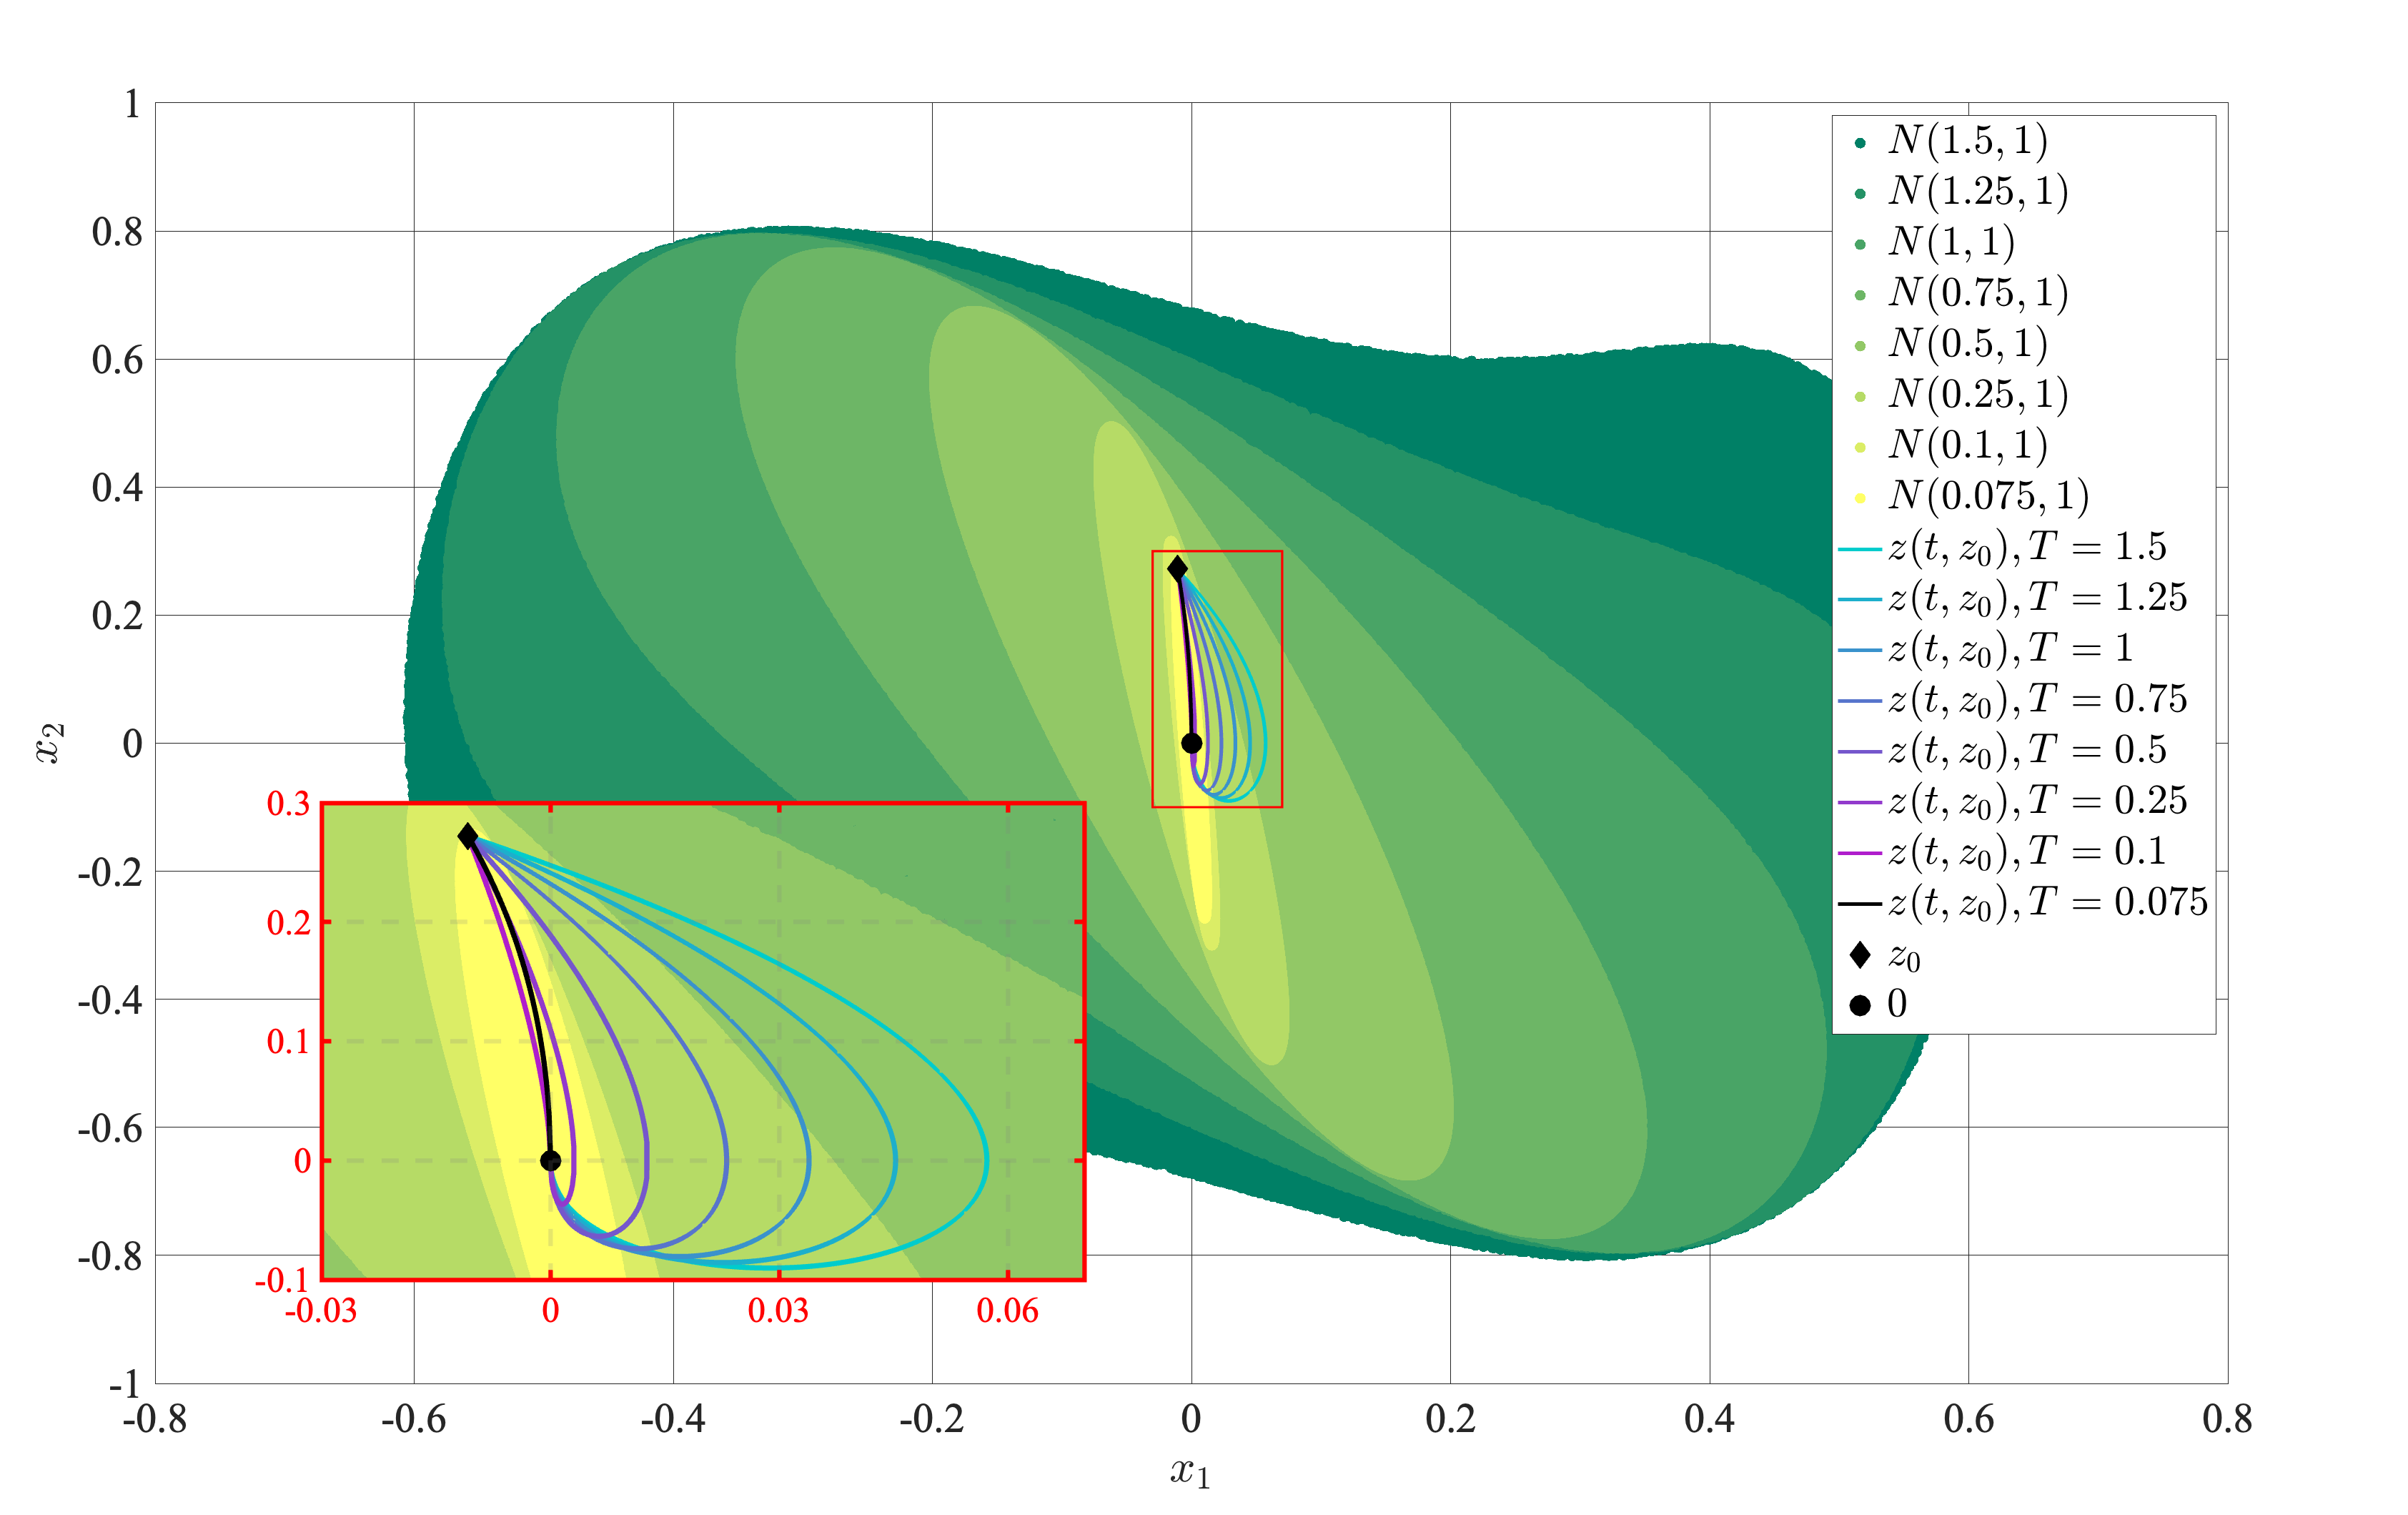
\includegraphics[width=\linewidth]{images/GusevMIOsipov_Duffing_fixed_z0.eps}
    \caption{Результаты экспериментов с переменным $T$.}
    \label{fig:series1}
\end{figure}

Несмотря на то, что условие $z_0 \in B(0,r_1(T))$ Теоремы \ref{th:tends_to_zero} не выполняется при $r_1(T)$, используемом в доказательстве, траектории по-прежнему стремятся к нулю. 
Это можно объяснить слишком строгим выбором $r_1(T)$ и тем, что теорема \ref{th:tends_to_zero} формулирует только достаточные условия для того, чтобы траектории стремились к нулю. 
Можно заметить, что в случае фиксированных начальных условий с уменьшением $T$ относительная разность функционалов $\Delta_J$ уменьшается, что следует из оценки, полученной в теореме \ref{th:functional_error_estimate}.

Теперь мы немного изменим условия эксперимента. 
Мы изменим не только $T$, но и начальные условия $z_0$ так, чтобы, во-первых, выполнялось равенство 
$z_0^{\top} Q_T(0) z_0 = 1$, а во-вторых, чтобы точка $z_0$ находилась внутри 
соответствующего множества нуль-управляемости $G_{-}(T,1)$.


\begin{table}
\caption{Результаты экспериментов с изменением $T$ и $z_0$}
\label{ExampleTable2}
\begin{center}
\begin{tabular}{c|c|c|c|c|c|c}
     № &    $T$  & $z_0$            & $\|z_0\|^2$&$z_0^{\top} Q_T(0) z_0$ &$J(T,z_0)$&$\Delta_J$ \\ \hline 
     1 &   1.500 & [-0.594;-0.057]  & 0.356680   & 0.999993    & 1.075833 & 0.0758407 \\ \hline
     2 &   1.250 & [-0.578;0.226]   & 0.385032   & 0.999997    & 1.110464 & 0.1104671 \\ \hline
     3 &   1.000 & [-0.502;0.508]   & 0.509514   & 0.999999    & 1.108159 & 0.1081607 \\ \hline
     4 &   0.750 & [-0.354;0.652]   & 0.550391   & 1.000000    & 1.048784 & 0.0487844 \\ \hline
     5 &   0.500 & [-0.195;0.638]   & 0.445513   & 1.000000    & 1.009848 & 0.0098475 \\ \hline
     6 &   0.250 & [-0.069;0.481]   & 0.236487   & 1.000000    & 1.000349 & 0.0003490 \\ \hline
\end{tabular}
\end{center}
\end{table} 

Результаты этой серии экспериментов 
показаны на рисунке \ref{fig:series2} и в таблице 
\ref{ExampleTable2}.
Зелеными областями обозначены множества нуль-управляемости $G_{-}(T,1)$ системы 
\eqref{Дуффинг} при $T = \{0.25, 0.5, 0.75, 1.0, 1.25, 1.5\}$, пунктирные линии 
линии показывают границы множества нуль-управляемости линеаризованной системы 
\eqref{LinearDuffing}, сплошные линии показывают траектории нелинейной системы 
при различных $T$. 
Символы "$\blacklozenge$" разных цветов обозначают 
начальные условия $z_0$, а "$\bullet$" --- целевую точку, расположенную в 
в начале координат. 

Замечание о невыполнении условия из первой части примера актуально и здесь. 
Из таблицы \ref{ExampleTable2} видно, что значения $\Delta_J$ также уменьшаются с уменьшением $T$, но это уменьшение не монотонно. 
По-видимому, это связано с тем, что меняется не только $T$, но и $z_0$.

\begin{figure}
    \centering
    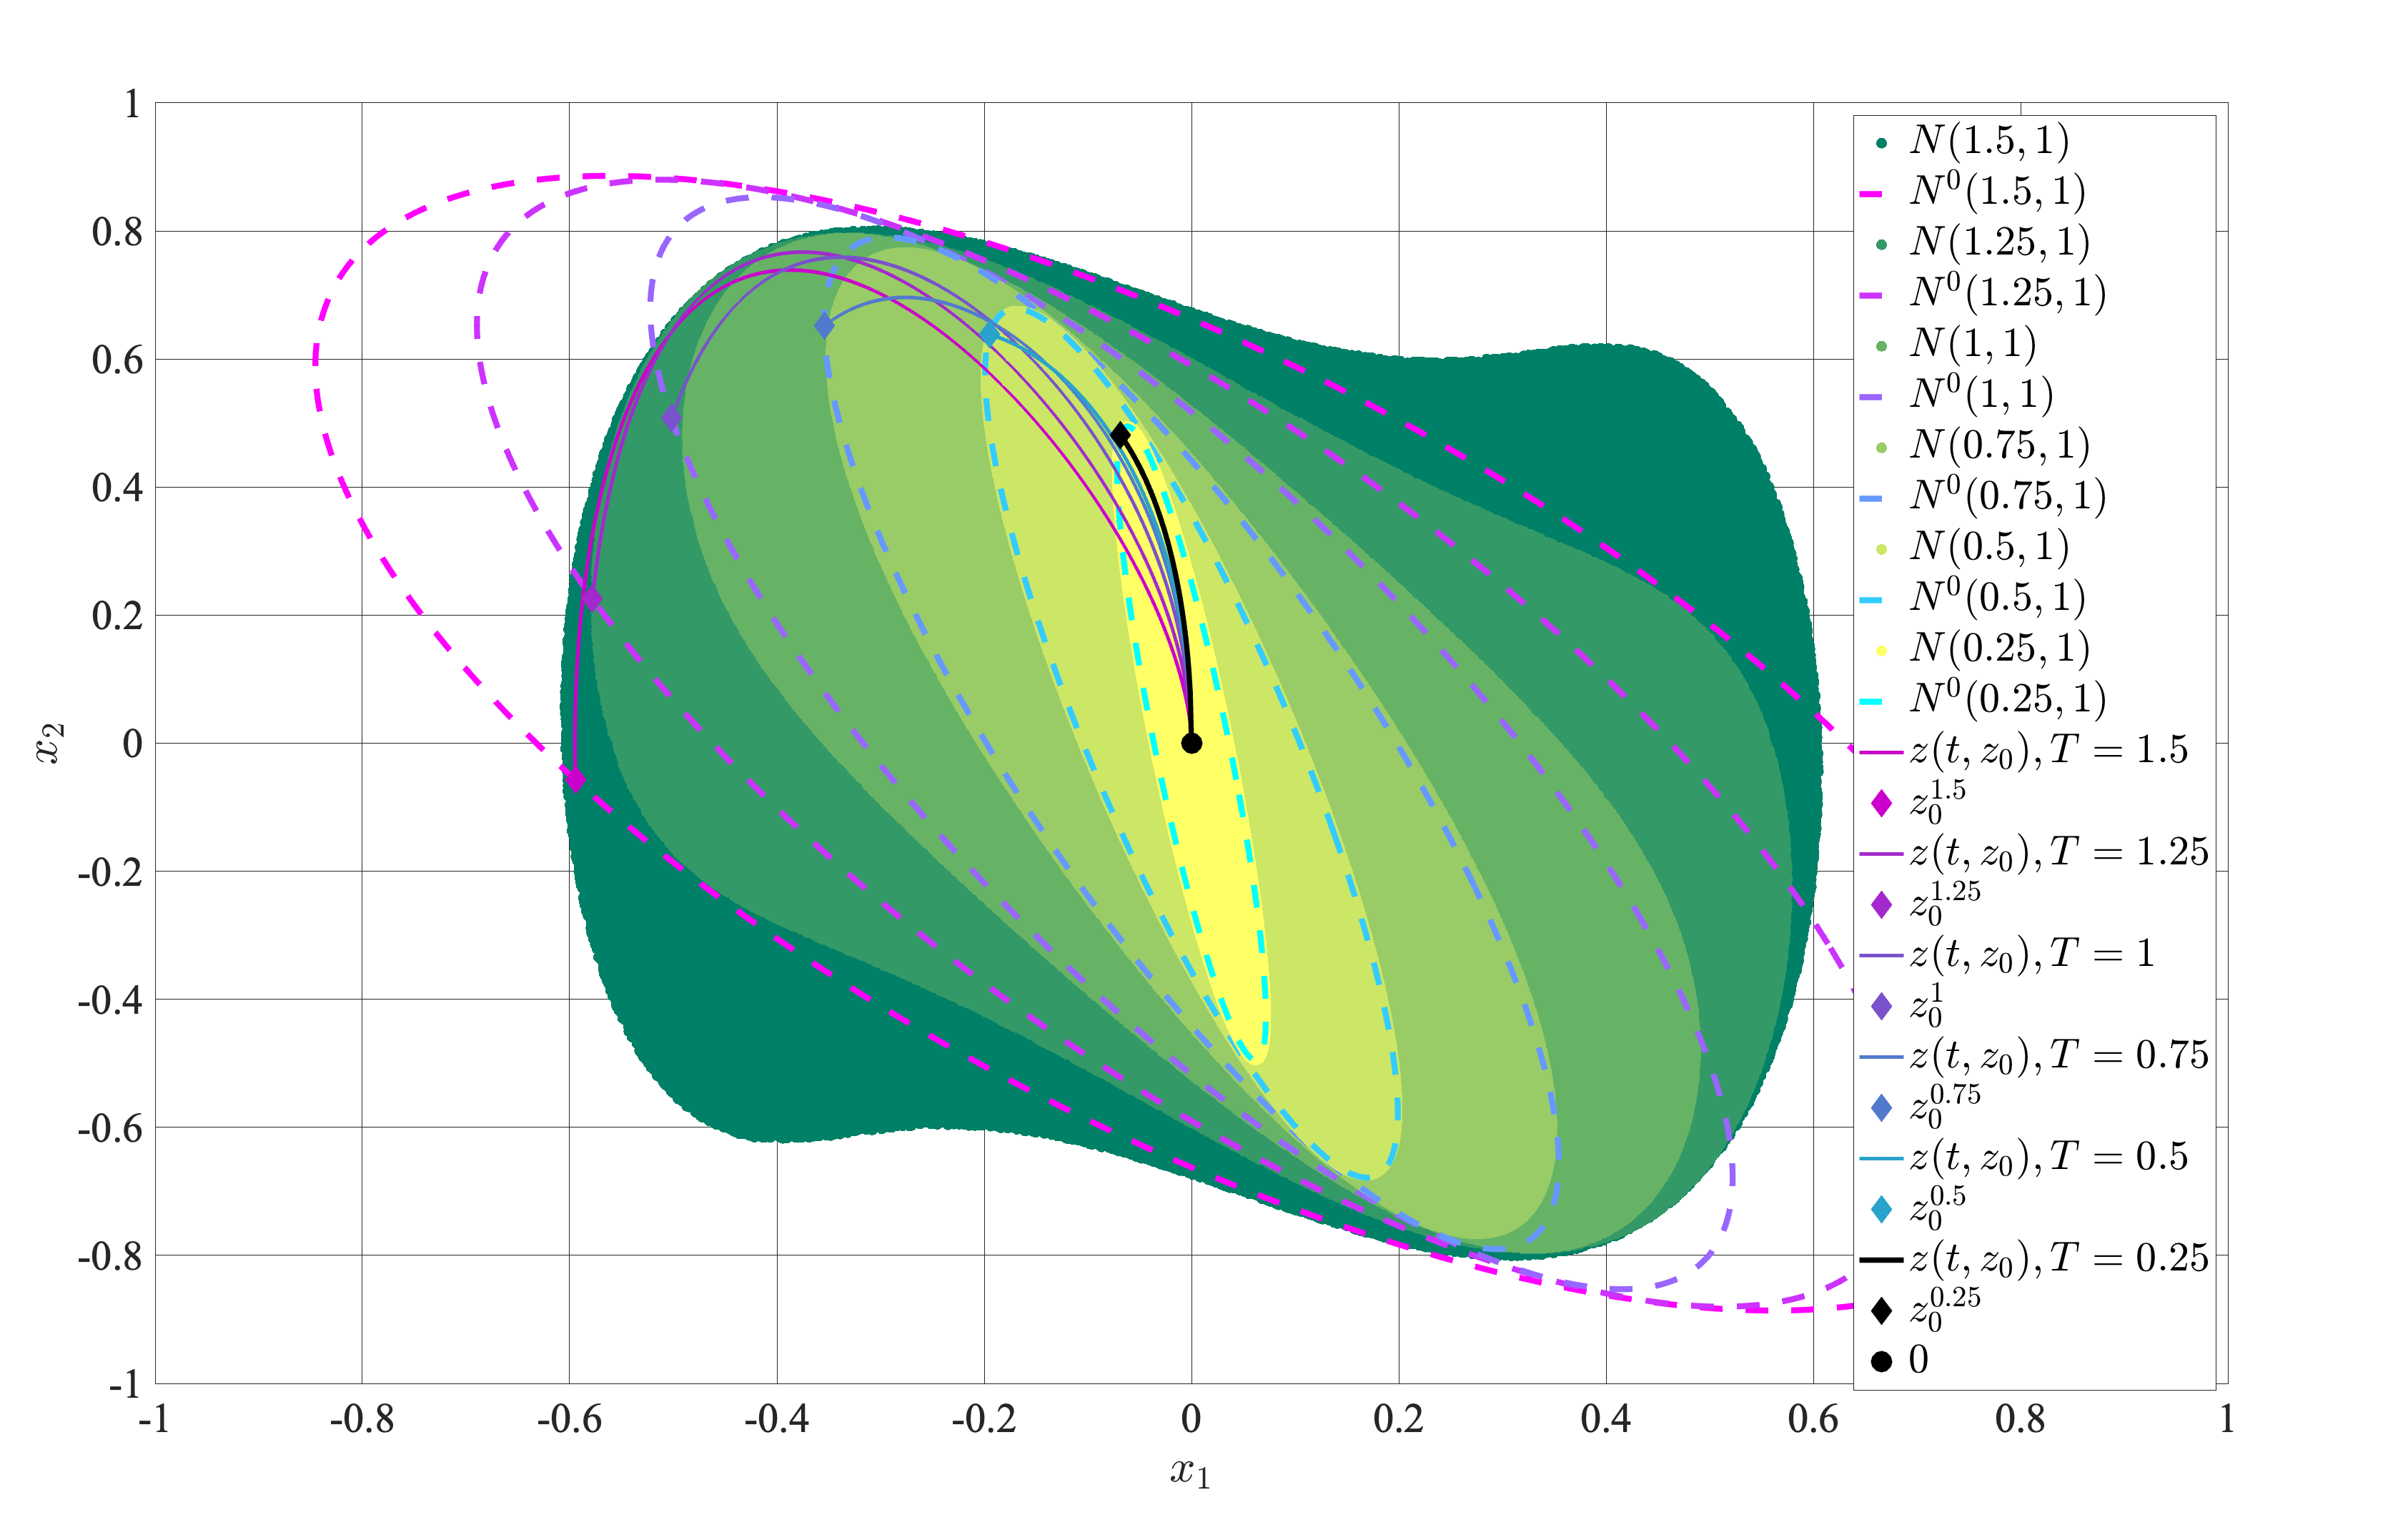
\includegraphics[width=\linewidth]{images/GusevMIOsipov_Duffing_variable_z0.eps}
    \caption{Результаты экспериментов с изменением $T$ и $z_0$}
    \label{fig:series2}
\end{figure}

Также на рисунке \ref{fig:series2} видно, что множества нуль-управляемости нелинейной и линеаризованной систем близки по форме при $ T \leqslant 0.75$. 

\subsubsection{Заключение}
Показано, что метод линеаризации может быть применен к задаче синтеза оптимального управления на конечном интервале времени. 
Линейная обратная связь, расчитанная для линеаризованной системы, также обеспечивает локальное решение задачи синтеза для нелинейной системы, если промежуток времени достаточно мал.   
Для этого требуются достаточно строгие ограничения на асимптотику грамиана управляемости, которые совпадают с достаточными условиями, обеспечивающими асимптотическую эквивалентность множеств достижимости (множеств нуль-управляемости). 
При этих условиях получена оценка для относительных значений погрешности интегрального функционала. 
Для демонстрации реализации описанного метода синтеза приведен пример нелинейной упругой системы под действием внешней силы. 

\end{document}